\section{Methods and Methodology}

\begin{figure}[!h]
    \centering
        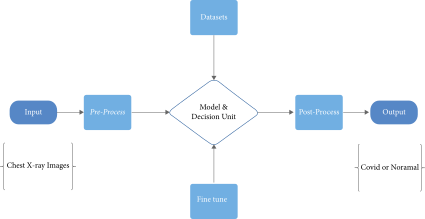
\includegraphics{assets/block.png}
    \caption{Block Diagram~\cite{Uddin2021} of the Proposed System}
\end{figure}

\subsection{Data Collection/Input:}

The data set is collected from different sources. We have proposed a framework that can effectively detect COVID-19 cases by evaluating the chest x-ray images. The image data are collected from different websites such as Radiopedia.org and Figure1.com. The random images are studied and divided into Normal image and Covid image. This data set is further converted into training and testing with the split of 70\% data for training of proposed deep learning model and 30\% data for testing purpose. 

\subsection{Data pre-processing }

Due to inconsistency of the dataset, the X-ray images are of different sizes. So, the all the images are converted to the same size. Also, splitting dataset process and data augmentation technique comes under data pre-processing. Final input to the proposed model is prepared. 

\begin{figure}
    \centering
        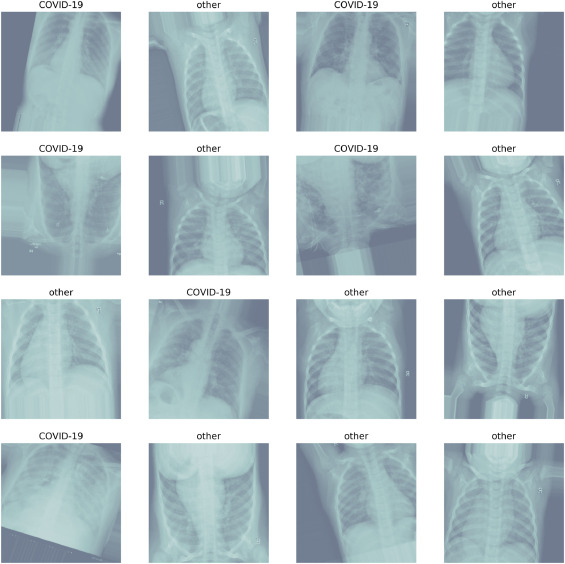
\includegraphics{assets/chest.png}
    \caption{Figure: Sample of the labelled X-rays after data augmentation taken from the combined data set of COVID-19 patients and normal patients }
\end{figure}

Algorithms: 

Convolutional Neural Network 

Convolutional Neural Network is one of the popular deep learning algorithms which are used for the analysis of image data. CNN make the use of learned features with input data, and uses convolutional layers, and make this architecture well suited for processing the images. 

 

 
\begin{figure}
    \centering
    \includegraphics{}
    \caption{Convolutional Neural Network}
\end{figure}
 

 
\begin{figure}
    \centering
    \includegraphics{}
    \caption{Convolutional Neural Network ~\cite{Uddin2021}}
\end{figure}

There are three types of layers in Convolutional Neural Networks.  

1) Convolutional Layer: The convolutional layer, considered as a main layer of a CNN, performs the operation called “convolution”. Kernels in the convolutional layer are applied to the layer inputs. In CNN, the input layer neurons is connected to the neuron hidden layer.  

2) Pooling Layer: The pooling layer is used to reduce the dimensionality of the feature map. There will be multiple activation & pooling layers inside the hidden layer of the CNN. 

3) Fully-Connected layer. The input to the fully connected layer is the output from the final Pooling or Convolutional Layer, which is flattened and then fed into the fully connected layer. 

 

 

 

 

 

3.Testing CNN: 

After making the model, the external X-ray images are tested using the classifier model. And the image is categorized as Covid infected or not. 

 

Classification Performance Evaluation: 

After diagnosing the X-rays in the test set, the propotion of each diagnosis is obtained. The performance evaluation indices are: 

Accuracy: 

Accuracy is a ratio of correctly predicted observation to the total observations. It is represented as: 

Accuracy = TP+TN/TP+FP+FN+TN 

Precision: 

Precision is the ratio of correctly predicted positive observations to the total predicted positive observations. High precision relates to the low false positive rate. It is represented as : 

Precision = TP/TP+FP 

Recall: 

Recall is the ratio of correctly predicted positive observations to the all observations in actual class. It is represented as: 

Recall = TP/TP+FP 

 